\documentclass{report}
\usepackage[spanish]{babel}
\usepackage[utf8]{inputenc}
\usepackage{graphicx, url, longtable, float, titlesec, hyperref, enumitem, verbatim, dingbat}
\usepackage[dvipsnames]{xcolor}
\usepackage[margin=4cm]{geometry}

\usepackage{enumitem,amssymb}
\newlist{todolist}{itemize}{2}
\setlist[todolist]{label=$\square$}
\usepackage{pifont}
\newcommand{\cmark}{\ding{51}}%
\newcommand{\xmark}{\ding{55}}%
\newcommand{\done}{\rlap{$\square$}{\raisebox{2pt}{\large\hspace{1pt}\cmark}}%
\hspace{-2.5pt}}
\newcommand{\wontfix}{\rlap{$\square$}{\large\hspace{1pt}\xmark}}

\usepackage{tabularx}
\usepackage{booktabs}

\title{Proyecto AS}
\author{Francisco Fernández Condado}
\date{November 2024}

\titleformat{\chapter}[display]
  {\normalfont\bfseries}{}{0pt}{\Huge}

\begin{document}
    \begin{titlepage}
        \centering
        
\includegraphics[width=0.7\linewidth]{img/bie.jpg}\\
        \vspace{3.5cm}
        \Huge Agenda cultural de Euskadi\\
        \vspace{2.5cm}
        \Large Administración de Sistemas\\
        \vspace{0.5cm}
        \large 4º Curso\\
        \vspace{3cm}
        \LARGE Grado en Ingeniería Informática de Gestión y Sistemas de Información\\
        \vspace{1cm}
        \large Francisco Fernández Condado\\
        \vspace{0.5cm}
        \large 24 de noviembre de 2024\\
    \end{titlepage}
    
    \tableofcontents
    
    \chapter{Introducción}
        Este proyecto propone la creación de una aplicación web funcional basándose en los contenedores de Docker y, de forma opcional, realizar el despliegue equivalente de Kubernetes.

        En este caso, la idea es crear un portal web interactivo que permita consultar la Agenda Cultural de Euskadi con actualizaciones en tiempo real. Para ello, se ha hecho uso de la información proporcionada en el \href{https://opendata.euskadi.eus/catalogo/-/kulturklik-agenda-cultural/}{portal Open Data del Servicio web del Gobierno Vasco}, que provee diferentes formas de acceso a la información completa.

        Se ha elegido hacer uso de un servidor web basado en nginx, que se encargará de redirigir las peticiones a un servidor Flask. La información de los eventos queda registrada en una base de datos PostgreSQL y, mediante un entorno adicional basado en Python, se actualizan los datos de los eventos a partir de la \href{https://opendata.euskadi.eus/apis/-/apis-open-data/}{API de Open Data} para contar con actualizaciones en tiempo real. Además, se cuenta con un entorno adicional que permite exportar los detalles de los eventos a un formato PDF, siendo más cómodo para imprimir o compartir en caso de ser necesario.

        \begin{figure}[H]
            \centering
            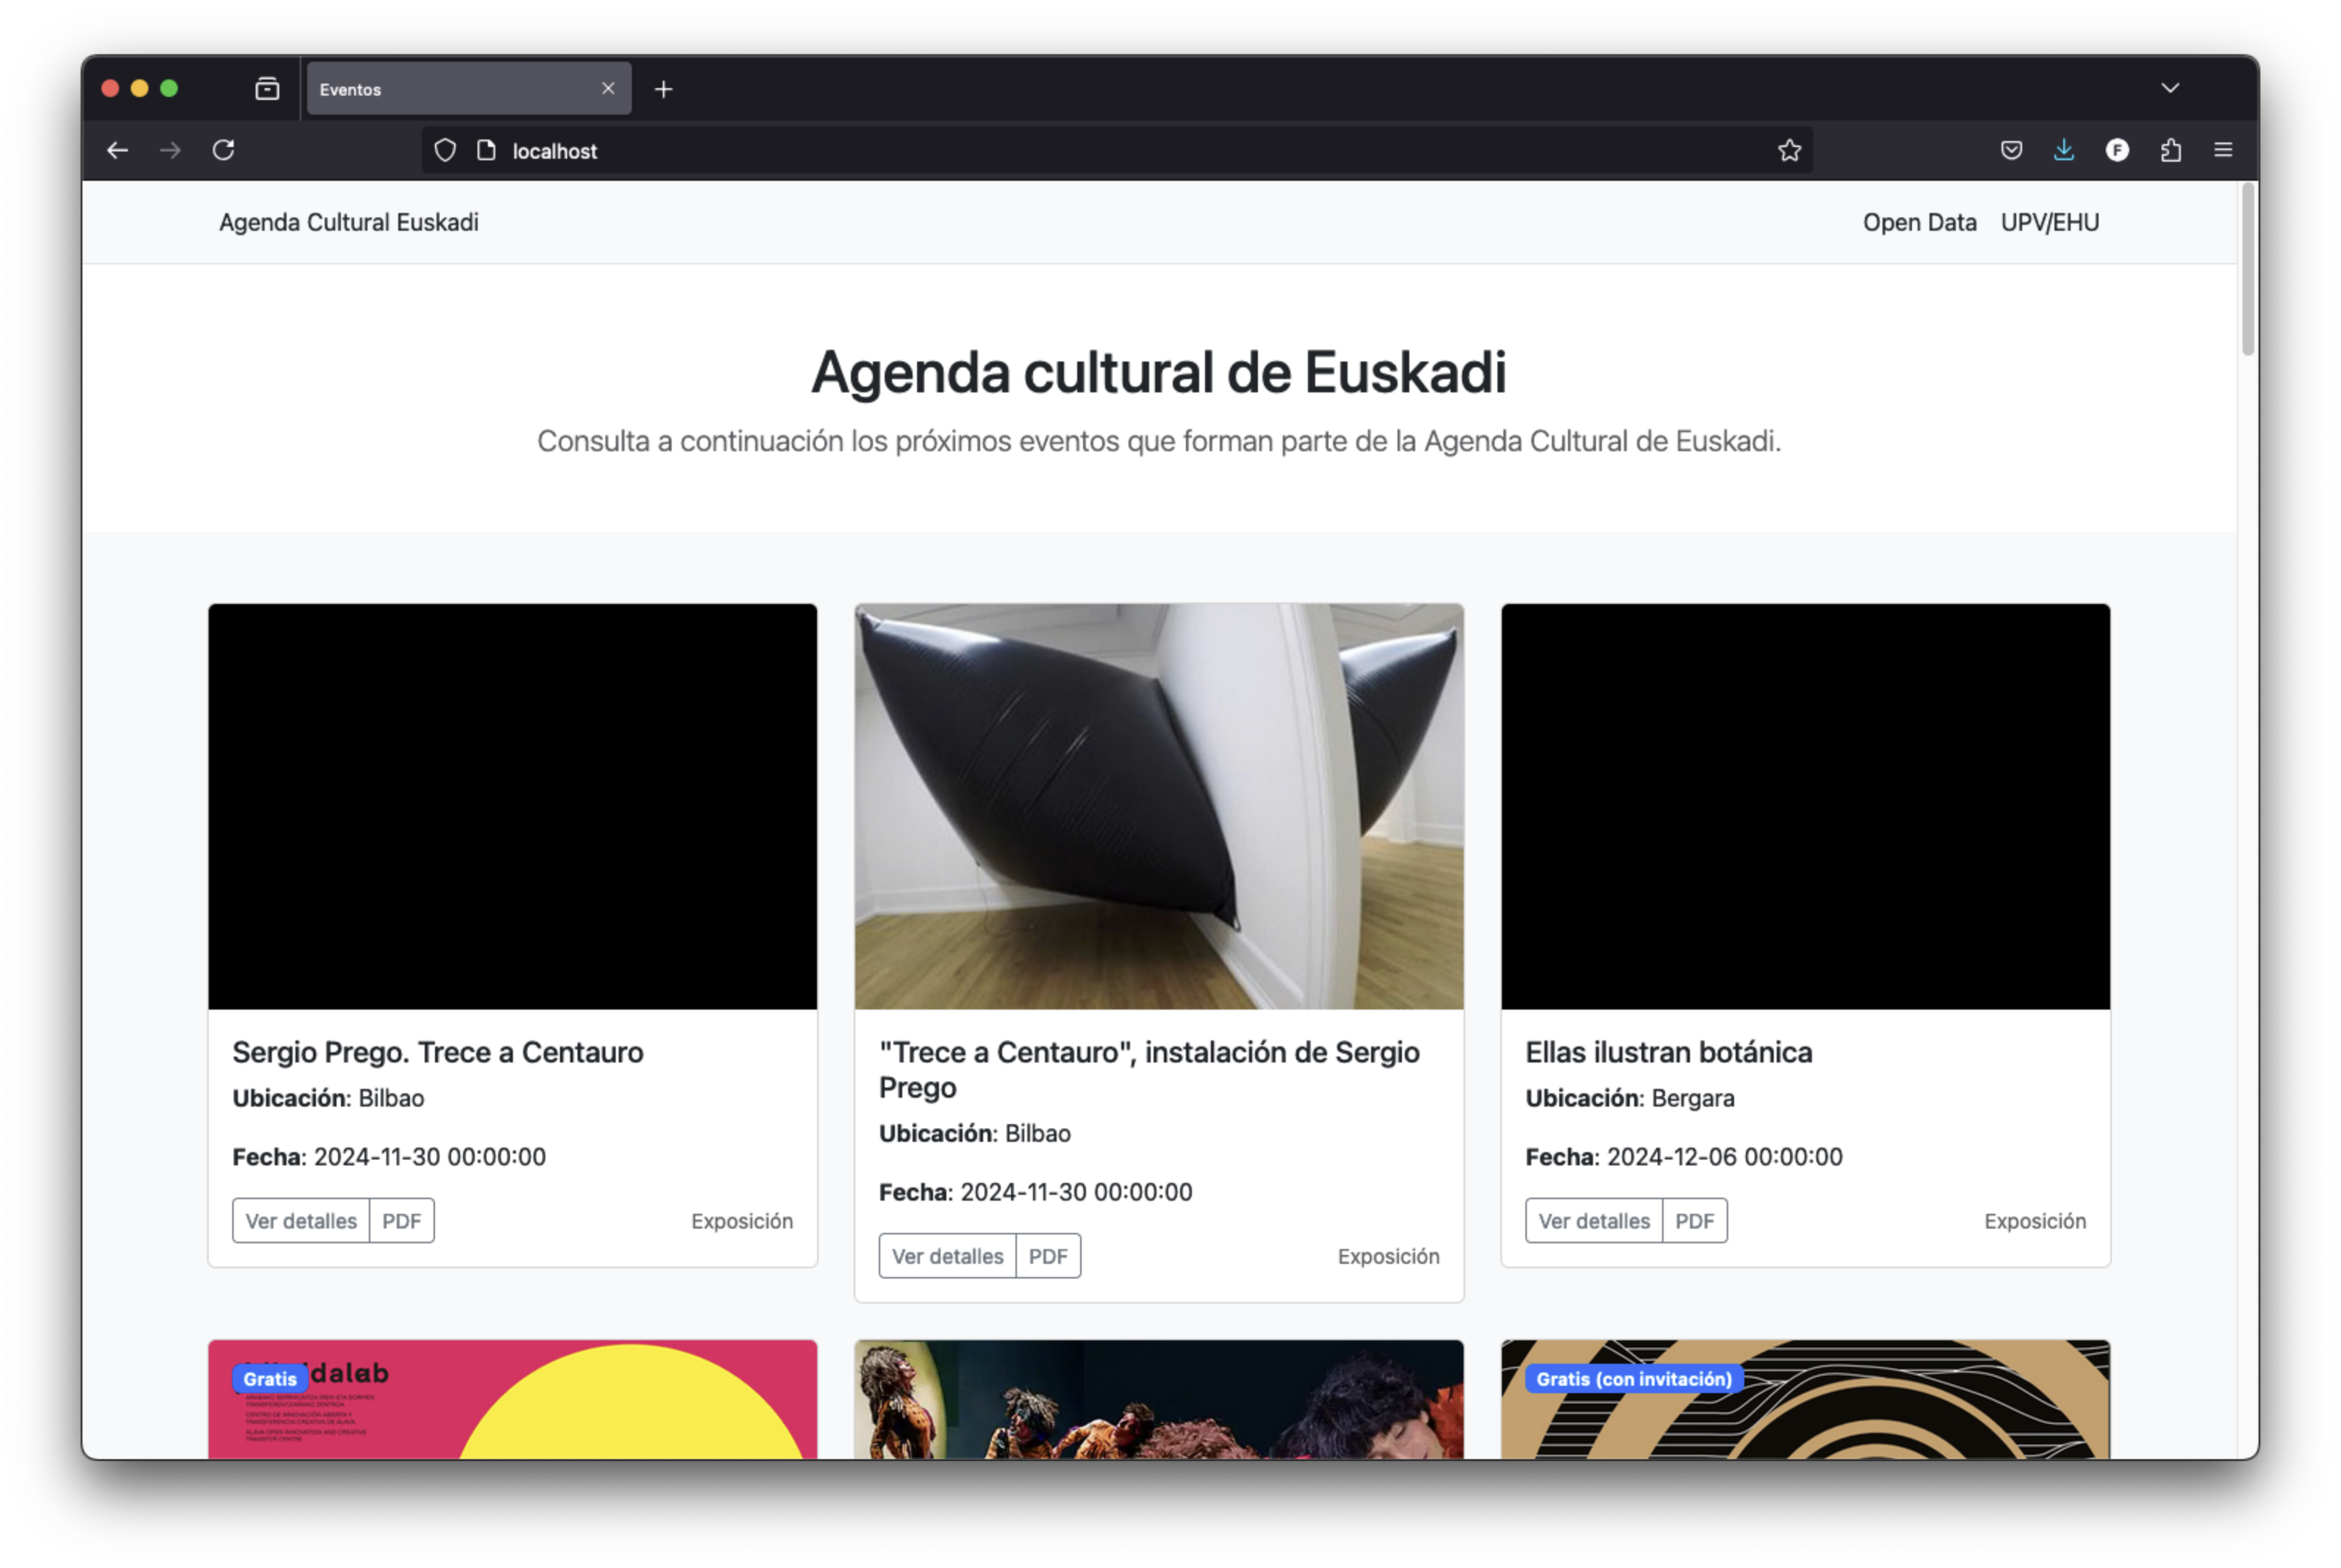
\includegraphics[width=0.8\linewidth]{img/general.png}
            \caption{Vista general de la aplicación}
            \label{fig:general}
        \end{figure}

        De este modo, la aplicación web permite acceder a un catálogo actualizado en tiempo real de los eventos presentes en la Agenda Cultural de Euskadi, con un diseño sencillo basado en la librería \href{https://getbootstrap.com}{Bootstrap}. Accediendo al detalle completo, será posible consultar toda la información (fechas, descripción, coste, categoría, lugar de realización, enlaces adicionales, etc.), así como a un mapa que muestra la ubicación en la que se realizará el evento.

        El despliegue completo de la aplicación puede encontrarse en el siguiente repositorio de GitHub para su uso y descarga: \url{https://github.com/ffernandezco/as_proyecto}.

    \chapter{Listado de tareas realizadas}

        \begin{itemize}
          \item Tareas obligatorias:
          \begin{todolist}
              \item[\done] Desarrollo de una aplicación funcional utilizando, al menos, un servidor web, un servidor de BBDD y una imagen a libre elección, basada en datos de repositorios públicos.
              \item[\done] Creación de las imágenes Docker necesarias para el proyecto, subiéndose a un repositorio público de Docker Hub.
              \item[\done] Creación de un entorno Docker Compose que permite ejecutar la aplicación desarrollada.
          \end{todolist}
          \item Tareas adicionales:
          \begin{todolist}
              \item[\done] Crear un despliegue Kubernetes que permita ejecutar la aplicación desarrollada.
              \item[\done] Inclusión de imágenes o contenedores adicionales que aporten nuevas funcionalidades a la aplicación sobre Docker Compose o Kubernetes.
              \item[\done] Uso de funcionalidades de Kubernetes no vistas en clase.
          \end{todolist}
        \end{itemize}

    \chapter{Instalación y despliegue del proyecto}
        El proyecto cuenta con un total del 6 servicios, que deben ser desplegados de forma conjunta con el fin de garantizar todas las funcionalidades disponibles:

        \begin{itemize}
            \item \textbf{Servicio \textit{nginx}}: propone el uso de un \href{https://nginx.org/en/}{servidor \textit{nginx}} con una configuración personalizada que redirige las peticiones al servicio Flask, sobre el que se hablará más adelante. Se basa en la última versión disponible en Docker Hub de la imagen: \url{https://hub.docker.com/_/nginx}.
            \item \textbf{Servicio \textit{postgres}}: construye un servidor de bases de datos \textit{\href{https://www.postgresql.org}{PostgreSQL}}, al que posteriormente se accederá mediante Flask para mostrar la información de los eventos, así como por el contenedor Python encargado de actualizar la información y por el gestor de bases de datos. Se basa en la última versión disponible en Docker Hub de la imagen: \url{https://hub.docker.com/_/postgres}.
            \item \textbf{Servicio \textit{adminer}}: aunque no aporta ninguna funcionalidad útil de cara al público, el \href{https://www.adminer.org}{gestor Adminer} permite de una forma sencilla gestionar las bases de datos del contenedor PostgreSQL mencionado anteriormente directamente desde una interfaz web basada en PHP. Se basa en la última versión disponible en Docker Hub de la imagen: \url{https://hub.docker.com/_/adminer/}.
            \item \textbf{Servicio \textit{updater}}: propone un contenedor basado en la última versión de la \href{https://hub.docker.com/_/python}{imagen de Python} que se encargará de ejecutar un script que, a través de la API de Open Data Euskadi, obtendrá los registros más recientes y actualizará la base de datos PostgreSQL mencionada anteriormente incluyendo los registros más recientes. Se trata de una imagen personalizada que, frente a la oficial, incluye la instalación de las librerías necesarias para que el script funcione, así como un \textit{cron} personalizado, que se encarga de comprobar si hay actualizaciones disponibles cada un minuto. Se puede consultar la imagen de forma pública en Docker Hub: \url{https://hub.docker.com/r/franciscofdez/updater-amd64}.
            \begin{itemize}
                \item La imagen fue creada originalmente en la arquitectura ARM, contando con disponibilidad limitada al ejecutarse en entornos AMD64: \url{https://hub.docker.com/r/franciscofdez/updater}
                \item Para ejecutarse en un entorno Kubernetes, se ha creado la siguiente imagen dedicada, que en este caso está optimizada para ser instanciada mediante un \textit{Cronjob} y, por tanto, son necesarios menos pasos para generarla: \url{https://hub.docker.com/r/franciscofdez/events-updater-2}
            \end{itemize}
            \item \textbf{Servicio \textit{flask}}: construye un segundo contenedor personalizado, de nuevo basado en la última versión de la \href{https://hub.docker.com/_/python}{imagen de Python}, que se encargará de porporcionar a nginx la salida necesaria según la consulta realizada sobre el puerto 80. En este caso, se ha optado por una imagen personalizada que instala las dependencias necesarias, incluyendo el \href{https://flask.palletsprojects.com/en/stable/}{motor Flask}, y que cuenta con un fichero \textit{app.py} que se encargará de gestionar las peticiones, bien por consultas a la base de datos PostgreSQL y ofreciendo salidas a través de las plantillas diseñadas, o bien realizando una solicitud al servicio Gotenberg que se expondrá a continuación. Se puede consultar la imagen de forma pública en Docker Hub: \url{https://hub.docker.com/r/franciscofdez/flask_app-amd64}.
            \begin{itemize}
                \item La imagen fue creada originalmente en la arquitectura ARM, contando con disponibilidad limitada al ejecutarse en entornos AMD64: \url{https://hub.docker.com/r/franciscofdez/flask_app}
                \item Para ejecutarse en un entorno Kubernetes, se ha creado la siguiente imagen dedicada: \url{https://hub.docker.com/r/franciscofdez/flask-k8s}
            \end{itemize}
            \item \textbf{Servicio \textit{gotenberg}}: se trata de una funcionalidad adicional añadida, que permite obtener la información de un evento en formato PDF. El servicio se basa en \href{https://gotenberg.dev}{el motor Gotenberg}, que permite crear una API sencilla para obtener ficheros en formato PDF. Las consultas a dicha API estarán gestionadas por el servicio Flask mencionado anteriormente, permitiendo al usuario final descargar cualquier fichero generado si así lo desea. Se basa en la versión 8 de la imagen oficial disponible en Docker Hub: \url{https://hub.docker.com/r/gotenberg/gotenberg/}.
        \end{itemize}

        En dos directorios separados, \textit{Docker} y \textit{Kubernetes}, se han incluido los ficheros necesarios para realizar el despliegue mediante Docker (con su entorno Compose), así como en Kubernetes. A continuación se exponen instrucciones dedicadas para ambos servicios.
        
        \section{Despliegue mediante Docker}

        El fichero \textit{docker-compose.yml} permite un despliegue automático a partir de las imágenes mencionadas anteriormente. Sin embargo, en primer lugar, será necesario crear un secreto, que se encargará de colocar la contraseña necesaria para la base de datos PostgreSQL. Dicho secreto será usado, además, por los contenedores de Flask y Python, que necesitarán acceder a la base de datos correspondiente.

        Para crear el secreto, basta con crear un fichero nuevo con el nombre \textit{postgres\_password} en el directorio \textit{secrets}. Asumiendo que primero se ha clonado el repositorio y que se ha realizado la instalación de Docker y Docker Compose en el equipo, ejecutando los siguientes comandos se puede replicar el escenario:

        \begin{verbatim}
    $ cd Docker
    $ mkdir secrets
    $ echo "micontraseña" > ./secrets/postgres_password
    $ docker compose up --build
        \end{verbatim}

        En concreto, el comando \textit{docker compose up --build}, permitirá crear una instancia completa a partir del fichero \textit{docker-compose.yml} En la \autoref{tab:docker} se exponen los diferentes servicios que este fichero pone en marcha al iniciar el contenedor, incluyendo los puertos que pueden usarse para consultar los diferentes servicios disponibles. Mencionar en este caso que, por cómo se ha generado, es posible que la primera vez que se realice el despliegue, se tarde unos minutos en poder ver la página principal hasta que el \textit{updater} se encargue de obtener los datos de la API de Open Data Euskadi.

        Una vez creado la primera vez, el despliegue pasa a ser más rápido, ya que además de los contenedores se ha definido el volumen \textit{postgres\_data} para almacenar los valores de la base de datos, de tal forma que después el \textit{updater} solo se encarga de actualizar la información.

        En este caso, todas las imágenes usadas están preparadas para poderse ejecutar de forma inmediata sin ningún fichero adicional, a excepción del contenedor \textit{nginx}. Para este contenedor, en el fichero \textit{/nginx/nginx.conf} se ha definido la configuración que debe usar el servidor para obtener las solicitudes de Flask y dirigirlas al puerto 80. Así, al acceder a la dirección IP del servidor o, en su defecto, a \textit{localhost}, cargará directamente la página principal.

        \begin{table}[H]
            \centering
            \begin{tabularx}{\textwidth}{lXrr}
                \toprule
                \textbf{Servicio} & \textbf{Imagen y descripción} & \textbf{Puerto original} & \textbf{Puerto expuesto} \\
                \midrule
                \\ \textbf{nginx} & {\parbox{5cm}{\\ \textit{\textbf{\href{https://hub.docker.com/_/nginx}{nginx:latest}}}\\Servidor basado en nginx. Redirige las peticiones solicitadas mediante la interfaz web al servicio correcto a partir del fichero \textit{/nginx/nginx.conf.}}} & 80 & 80 \\
                
                \\ \textbf{postgres} & {\parbox{5cm}{\textit{\textbf{\href{https://hub.docker.com/_/postgres}{postgres:latest}}} \\ Servidor de base de datos basado en PostgreSQL, usado para almacenar la información de los eventos. Crea automáticamente un usuario y una base de datos con la contraseña definida en el secreto correspondiente.}} & 5432 & 5432 \\
                \\ \textbf{adminer} & {\parbox{5cm}{\textit{\textbf{\href{https://hub.docker.com/_/adminer/}{adminer:latest}}}\\ Permite gestionar desde una interfaz visual la base de datos PostgreSQL mencionada anteriormente.}} & 8080 & 8081 \\
                \\ \textbf{updater} & {\parbox{5cm}{\textit{\textbf{\href{https://hub.docker.com/r/franciscofdez/updater-amd64}{franciscofdez/updater-amd64:latest}}} \\ Contenedor basado en Python que realiza, de forma periódica, consultas a la API de Open Data Euskadi para descargar los eventos más recientes de la agenda cultural.}} & -- & -- \\
                \\ \textbf{flask} & {\parbox{5cm}{\textbf{\textit{\href{https://hub.docker.com/r/franciscofdez/flask_app-amd64}{franciscofdez/flask\_app-amd64:latest}}} \\ Contenedor basado en Python con Flask usado para mostrar los detalles de los eventos en base a plantillas diseñadas con Bootstrap y dirigir las solicitudes a los servicios adecuados.}} & 5000 & 5001 \\
                \\ \textbf{gotenberg} & {\parbox{5cm}{\textit{\textbf{\href{https://hub.docker.com/r/gotenberg/gotenberg}{gotenberg/gotenberg:8}}} \\ Permite, mediante una API, realizar múltiples acciones relacionadas con documentos PDF. Se usa para convertir ficheros HTML con información sobre los eventos en este formato.}} & 3000 & 3000 \\
                \bottomrule
            \end{tabularx}
        \caption{Servicios definidos en el despliegue mediante Docker Compose}
        \label{tab:docker}
        \end{table}

        En lo que respecta a las imágenes propias, su código fuente se encuentra en el directorio anexo \textit{docker-images}, y pueden clonarse de forma directa al estar disponibles de forma pública en Docker Hub. A continuación se expone cómo han sido creadas y su funcionalidad en el proyecto:

        \subsection{Imagen \textit{updater}}

            El propósito de esta imagen es recoger, a partir de la API de Open Data Euskadi, los datos correspondientes a la agenda cultural del año en curso. Para gestionar esto, a partir de la imagen \textit{\href{https://hub.docker.com/_/python}{python:latest}}, se crea un contenedor en el que se instalan las dependencias \textit{requests}, \textit{psycopg2} y \textit{datetime}, necesarias para ejecutar el código del programa, que se encuentra descrito en el fichero \textit{main.py}.
    
            Para gestionar la actualización automática, se cuenta con el siguiente fichero \textit{crontab} personalizado, que se encarga de ejecutar el script cada minuto con el fin de comprobar si hay o no actualizaciones disponibles a partir de la API del Gobierno Vasco:
    
            \begin{verbatim}
    * * * * * root POSTGRES_PASSWORD_FILE=/run/secrets/postgres_password
    /usr/local/bin/python /app/main.py >> /var/log/cron.log 2>&1
            \end{verbatim}
    
            Por la estructura del contenedor, se deben especificar las variables de entorno en el propio fichero del cron. Además, dejaremos el resultado en un fichero \textit{cron.log} para poder depurar errores. Toda esta configuración se expresa en el fichero \textit{Dockerfile} usado para crear la imagen.

        \subsection{Imagen \textit{flask\_app}}

            La imagen personalizada \textit{flask\_app} se encarga de controlar un servidor basado en Flask, que se usará de cara al frontend de la aplicación. Para ello, se parte de nuevo de la imagen \textit{\href{https://hub.docker.com/_/python}{python:latest}}. A continuación, se realiza la instalación de las dependencias \textit{Flask}, \textit{flask-cors}, \textit{psycopg2} y \textit{requests}. Estas dependencias serán usadas por el fichero \textit{app.py}, que será el encargado de proporcionar las funcionalidades de Flask.

            En el directorio \textit{/templates}, se cuenta con diferentes plantillas, que serán las que tome en cuenta Flask. Además, es el encargado de gestionar las consultas del frontend a la base de datos PostgreSQL, así como de las solicitudes a la API de Gotenberg en el caso de que el usuario solicite un documento PDF.

            El fichero \textit{Dockerfile} se encargará de gestionar todo esto, instalando todo lo necesario e iniciando \textit{app.py} como es debido. Por cómo está construida la imagen, será necesario especificar en dicho fichero las variables de entorno que Flask necesitará más adelante.

        \section{Despliegue mediante Kubernetes}

            De cara al despliegue utilizando Kubernetes, la instanciación no es tan rápida como mediante Docker, al ser necesario configurar cada uno de los objetos de tipo ConfigMap, Deployment, Service, CronJob e Ingress que se han implementado.

            En este caso, se ha optado por realizar el despliegue en un entorno local, desplegado haciendo uso del motor de Kubernetes incluido en Docker Desktop, sobre el que puede obtenerse más información en \href{https://docs.docker.com/desktop/features/kubernetes/}{su sitio web oficial}. Además, los accesos han sido configurados a partir de la red con subdominios del tipo \textit{localdev.me} con propósitos de pruebas, si bien podría ajustarse para responder a otros dominios en un entorno basado en la nube.

            El motivo principal por el que se ha optado por realizar el despliegue haciendo uso de un entorno local guarda relación con el coste de la implementación en otros entornos como \textit{\href{https://cloud.google.com/kubernetes-engine/pricing}{Google Kubernetes Engine}}. Al hacer uso de un cluster de tipo \textit{Autopilot}, que gestionará de forma automática los contenedores y la creación de las máquinas, y al tener en este caso 5 máquinas funcionando en todo momento y una que se ejecuta de forma periódica haciendo uso de un objeto \textit{CronJob}, el coste podría dispararse. No obstante, en un entorno de producción, resulta una opción recomendable que facilita la implementación.

            Teniendo en cuenta estos detalles, para poder comenzar será necesario crear un secreto que contenga el nombre de usuario de la base de datos PostgreSQL así como su contraseña. Para hacer esto, debemos ejecutar el siguiente comando en nuestro entorno, sustituyendo \textit{"micontraseña"} por la contraseña deseada:

            \begin{verbatim}
    $ kubectl create secret generic postgres-secret \
    $ --from-literal=POSTGRES_USER="as" \
    $ --from-literal=POSTGRES_PASSWORD="micontraseña"
            \end{verbatim}

            A continuación, para poder crear una instancia básica del proyecto, será necesario ir ejecutando cada uno de los siguientes comandos sobre el directorio, que se encargan de configurar cada uno de los ficheros creados y, además, configurará el controlador de nginx necesario para ejecutar correctamente la configuración del Ingress para la red:

            \begin{verbatim}
    $ kubectl apply -f postgres-configmap.yaml
    $ kubectl apply -f postgres-pvc.yaml
    $ kubectl apply -f postgres-deployment.yaml
    $ kubectl apply -f postgres-service.yaml
    $ kubectl apply -f adminer-deployment.yaml
    $ kubectl apply -f adminer-service.yaml
    $ kubectl apply -f updater-cronjob.yaml
    $ kubectl apply -f gotenberg-deployment.yaml
    $ kubectl apply -f gotenberg-service.yaml
    $ kubectl apply -f flask-deployment.yaml
    $ kubectl apply -f flask-service.yaml
    $ kubectl apply -f nginx-configmap.yaml
    $ kubectl apply -f nginx-deployment.yaml
    $ kubectl apply -f nginx-service.yaml
    $ kubectl apply -f https://raw.githubusercontent.com/kubernetes/
    ingress-nginx/controller-v1.11.3/deploy/static/provider/cloud/
    deploy.yaml
    $ kubectl apply -f ingress.yaml
            \end{verbatim}

            Una vez realizado, ejecutando el comando \textit{kubectl get pods} podrán verse los diferentes contenedores creados, mientras que \textit{kubectl get jobs} devolverá las tareas del \textit{updater} definido en el CronJob correspondiente, y \textit{kubectl get ingress} mostrará la configuración de la red. Si todo ha funcionado de forma correcta, debería mostrarse algo similar a lo expuesto en la \autoref{fig:objetos-kubernetes}.

            \begin{figure}[H]
                \centering
                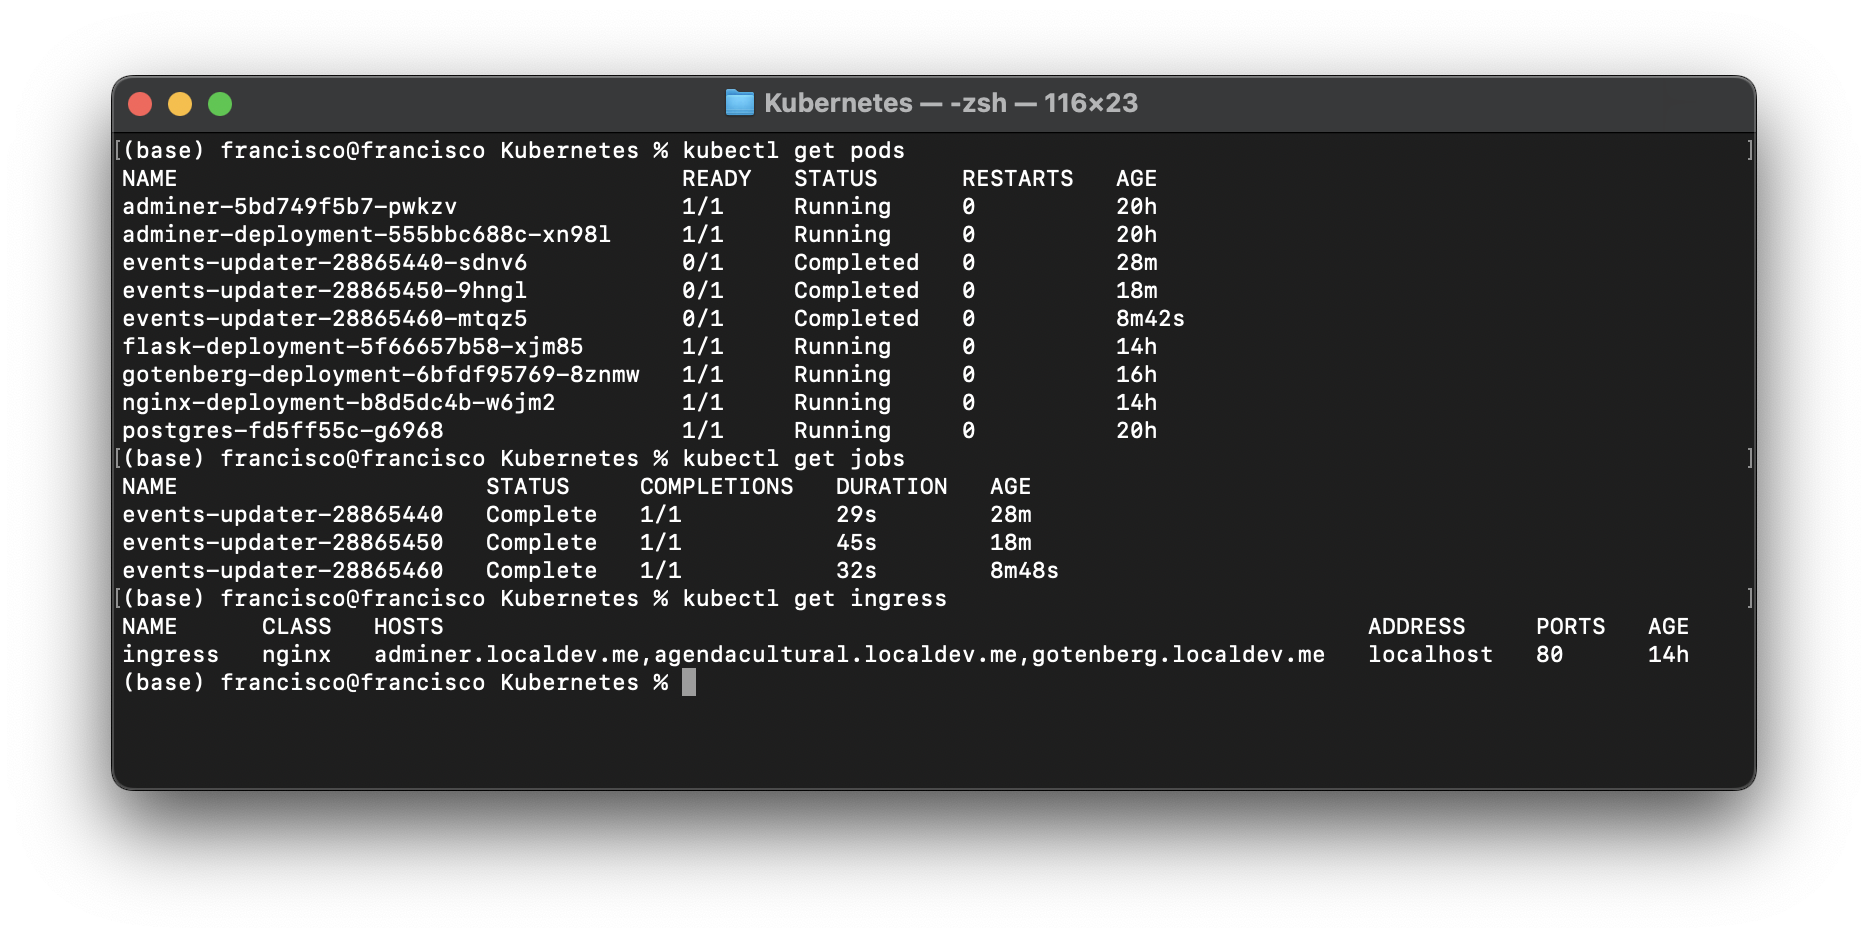
\includegraphics[width=1\linewidth]{img/despliegue-kubernetes.png}
                \caption{Objetos instanciados por Kubernetes}
                \label{fig:objetos-kubernetes}
            \end{figure}

            A continuación se expone cada uno de los ficheros de configuración que han sido utilizados para lograr el despliegue equivalente en Kubernetes, explicando su funcionalidad:

            \begin{itemize}
                \item \textbf{Servidor PostgreSQL}:
                \begin{itemize}
                    \item \textit{\textbf{postgres-configmap.yaml}}: define las variables necesarias para el servidor de la base de datos PostgreSQL, encargándose de crear una base de datos con el nombre "\textit{database}" y de definir "\textit{as}" como el nombre de usuario por defecto.
                    \item \textit{\textbf{postgres-pvc.yaml}}: se encarga de realizar la reclamación de volumen persistente para el servidor de la base de datos.
                    \begin{itemize}
                        \item \textbf{Modo de acceso}: se ha definido como \textit{ReadWriteOnce} para permitir el funcionamiento correcto de PostgreSQL.
                        \item \textbf{Almacenamiento}: se ha definido 1 GB de espacio en el campo \textit{storage}, que debería ser suficiente para almacenar la base de datos completa.
                    \end{itemize}
                    \item \textit{\textbf{postgres-deployment.yaml}}: define el funcionamiento general del servidor PostgreSQL, de acuerdo a las características detalladas a continuación.
                    \begin{itemize}
                        \item \textbf{Imagen base}: \href{https://hub.docker.com/_/postgres}{postgres:latest}
                        \item \textbf{Número de réplicas}: 1
                        \item Utiliza el secreto creado anteriormente como contraseña para la base de datos generada, así como la reclamación de volumen del campo anterior para almacenar la información.
                    \end{itemize}
                    \item \textit{\textbf{postgres-service.yaml}}: gestiona el servicio a través del que será posible acceder al contenedor.
                    \begin{itemize}
                        \item \textbf{Puerto de origen}: 5432
                        \item \textbf{Puerto de salida}: 5432
                    \end{itemize}
                \end{itemize}
                \item \textbf{Servicio Adminer}:
                \begin{itemize}
                    \item \textit{\textbf{adminer-deployment.yaml}}: gestiona el funcionamiento general del servicio Adminer, usado para gestionar visualmente la base de datos. Se basa en las características detalladas a continuación.
                    \begin{itemize}
                        \item \textbf{Imagen base}: \href{https://hub.docker.com/_/adminer/}{adminer:latest}
                        \item \textbf{Número de réplicas}: 1
                        \item Define el servidor por defecto de la base de datos como \textit{postgres-service}, ruta definida por el servicio PostgreSQL.
                    \end{itemize}
                    \item \textit{\textbf{adminer-service.yaml}}: se encarga de gestionar el servicio a través del que será posible acceder al contenedor.
                    \begin{itemize}
                        \item \textbf{Puerto de origen}: 8080
                        \item \textbf{Puerto de salida}: 30001
                        \item \textit{Se ha modificado el puerto de salida con respecto al despliegue de Docker por no dar problemas de compatibilidad con el despliegue de Kubernetes.}
                    \end{itemize}
                \end{itemize}
                \item \textbf{Servicio Updater}
                \begin{itemize}
                    \item \textit{\textbf{updater-cronjob.yaml}}: define un objeto de tipo \textit{Cronjob}, \textit{\textbf{funcionalidad de Kubernetes no vista en clase}}, que se encargará de instanciar, cada 10 minutos, el servicio de actualización de datos de acuerdo con las siguientes configuraciones.
                    \begin{itemize}
                        \item \textbf{Imagen base (propia)}: \href{https://hub.docker.com/r/franciscofdez/events-updater-2}{franciscofdez/events-updater-2:latest}. Se utiliza una imagen diferente a la de Docker pero con la misma funcionalidad, debido a que no es necesario configurar un \textit{cronjob} al usar, en su lugar, la funcionalidad de Kubernetes, así como para adaptarse a la forma de gestionar los secretos.
                        \item Utiliza como parámetros los datos de la base de datos del servicio PostgreSQL para conectarse, así como el secreto configurado previamente.
                    \end{itemize}
                \end{itemize}
                \item \textbf{Servicio Gotenberg}
                \begin{itemize}
                    \item \textit{\textbf{gotenberg-deployment.yaml}}: configura el funcionamiento general del servicio Gotenberg, usado para la generación de documentos PDF, de acuerdo con las características detalladas a continuación.
                    \begin{itemize}
                        \item \textbf{Imagen base}: \href{https://hub.docker.com/r/gotenberg/gotenberg/}{gotenberg/gotenberg:8}
                        \item \textbf{Número de réplicas}: 1
                    \end{itemize}
                    \item \textit{\textbf{gotenberg-service.yaml}}: se encarga de gestionar el servicio a través del que será posible acceder al contenedor.
                    \begin{itemize}
                        \item \textbf{Puerto de origen}: 3000
                        \item \textbf{Puerto de salida}: 30001
                        \item \textit{Se ha modificado el puerto de salida con respecto al despliegue de Docker por no dar problemas de compatibilidad con el despliegue de Kubernetes.}
                    \end{itemize}
                \end{itemize}
                \item \textbf{Servicio Flask}
                \begin{itemize}
                    \item \textit{\textbf{flask-deployment.yaml}}: objeto encargado de gestionar el contenedor, basado en Flask, que se mostrará en el frontend de la aplicación. Se encarga de mostrar, en base a las plantillas ya creadas, el contenido de la base de datos, o de llamar al servicio Gotenberg cuando un usuario solicita la creación de un documento PDF.
                    \begin{itemize}
                        \item \textbf{Imagen base (propia)}: \href{https://hub.docker.com/r/franciscofdez/flask-k8s}{franciscofdez/flask-k8s:latest}. Se utiliza una imagen diferente a la de Docker pero con la misma funcionalidad, debido a cómo funciona el entorno Python en Kubernetes, así como para adaptarse a la forma de gestionar los secretos.
                        \item \textbf{Número de réplicas}: 1
                        \item Utiliza como parámetros los datos de la base de datos del servicio PostgreSQL para conectarse, así como el secreto configurado previamente.
                    \end{itemize}
                    \item \textit{\textbf{flask-service.yaml}}: tiene como finalidad gestionar el servicio a través del que será posible acceder al contenedor Flask a partir de nginx o de forma directa.
                    \begin{itemize}
                        \item \textbf{Puerto de origen}: 5000
                        \item \textbf{Puerto de salida}: 30002
                        \item \textit{Se ha modificado el puerto de salida con respecto al despliegue de Docker por no dar problemas de compatibilidad con el despliegue de Kubernetes.}
                    \end{itemize}
                \end{itemize}
                \item \textbf{Servicio nginx}
                \begin{itemize}
                    \item \textit{\textbf{nginx-configmap.yaml}}: se encarga de configurar los parámetros necesarios de cara al servidor nginx. Contiene los mismos datos almacenados previamente en el fichero \textit{nginx.conf} de Docker.
                    \item \textit{\textbf{nginx-deployment.yaml}}: objeto encargado de gestionar el servidor nginx, que se usará para realizar consultas al contenedor de Flask cuando sea necesario.
                    \begin{itemize}
                        \item \textbf{Imagen base}: \href{https://hub.docker.com/_/nginx}{nginx:latest}.
                        \item \textbf{Número de réplicas}: 1
                    \end{itemize}
                    \item \textit{\textbf{nginx-service.yaml}}: se encarga de exponer el servidor nginx al exterior, usando para ello el puerto 80 por ser el predefinido para tráfico web HTTP.
                    \begin{itemize}
                        \item \textbf{Puerto de origen}: 80
                        \item \textbf{Puerto de destino}: 80
                    \end{itemize}
                \end{itemize}
                \item \textbf{Configuración de red}
                \begin{itemize}
                    \item \textit{\textbf{ingress.yaml}}: objeto encargado de gestionar la conectividad de los diferentes contenedores. Está optimizado para desarrollo local, por lo que se utilizan los siguientes dominios.
                    \begin{itemize}
                        \item \textit{adminer.localdev.me}: apunta al servicio Adminer.
                        \item \textit{agendacultural.localdev.me}: apunta al servicio Flask de forma directa, cargando la página principal.
                        \item \textit{gotenberg.localdev.me}: apunta directamente al servicio Gotenberg, pudiendo usarse a partir de su API propia.
                    \end{itemize}
                \end{itemize}
            \end{itemize}

    \chapter{Manual de uso y funcionalidades disponibles}

        Accediendo a la página principal, se mostrará automáticamente un listado completo de los eventos de la Agenda Cultural de Euskadi. Como se puede ver en la \autoref{fig:manual-1} cada uno de ellos, se verán algunos datos básicos, incluyendo el tipo, el nombre, la fecha, el lugar o una imagen.

        \begin{figure}[H]
            \centering
            
\includegraphics[width=0.9\linewidth]{img/manual-1.png}
            \caption{Página principal de la aplicación web}
            \label{fig:manual-1}
        \end{figure}

        Pulsando el botón de “Ver detalles”, será posible acceder a la página de detalles de los eventos, tal y como se muestra en la \autoref{fig:manual-2}. El contenido depende en este caso de la información proporcionada por la API de Open Data Euskadi para el evento en cuestión. Si contiene campos como el precio o un enlace recomendado se mostrarán. Además, de cara a los eventos con una localización asociada, se mostrará el mapa correspondiente, basado en los mapas de \href{https://www.openstreetmap.org}{OpenStreetMap} y \href{https://leafletjs.com}{Leaflet} para su consulta.

        \begin{figure}[H]
            \centering
            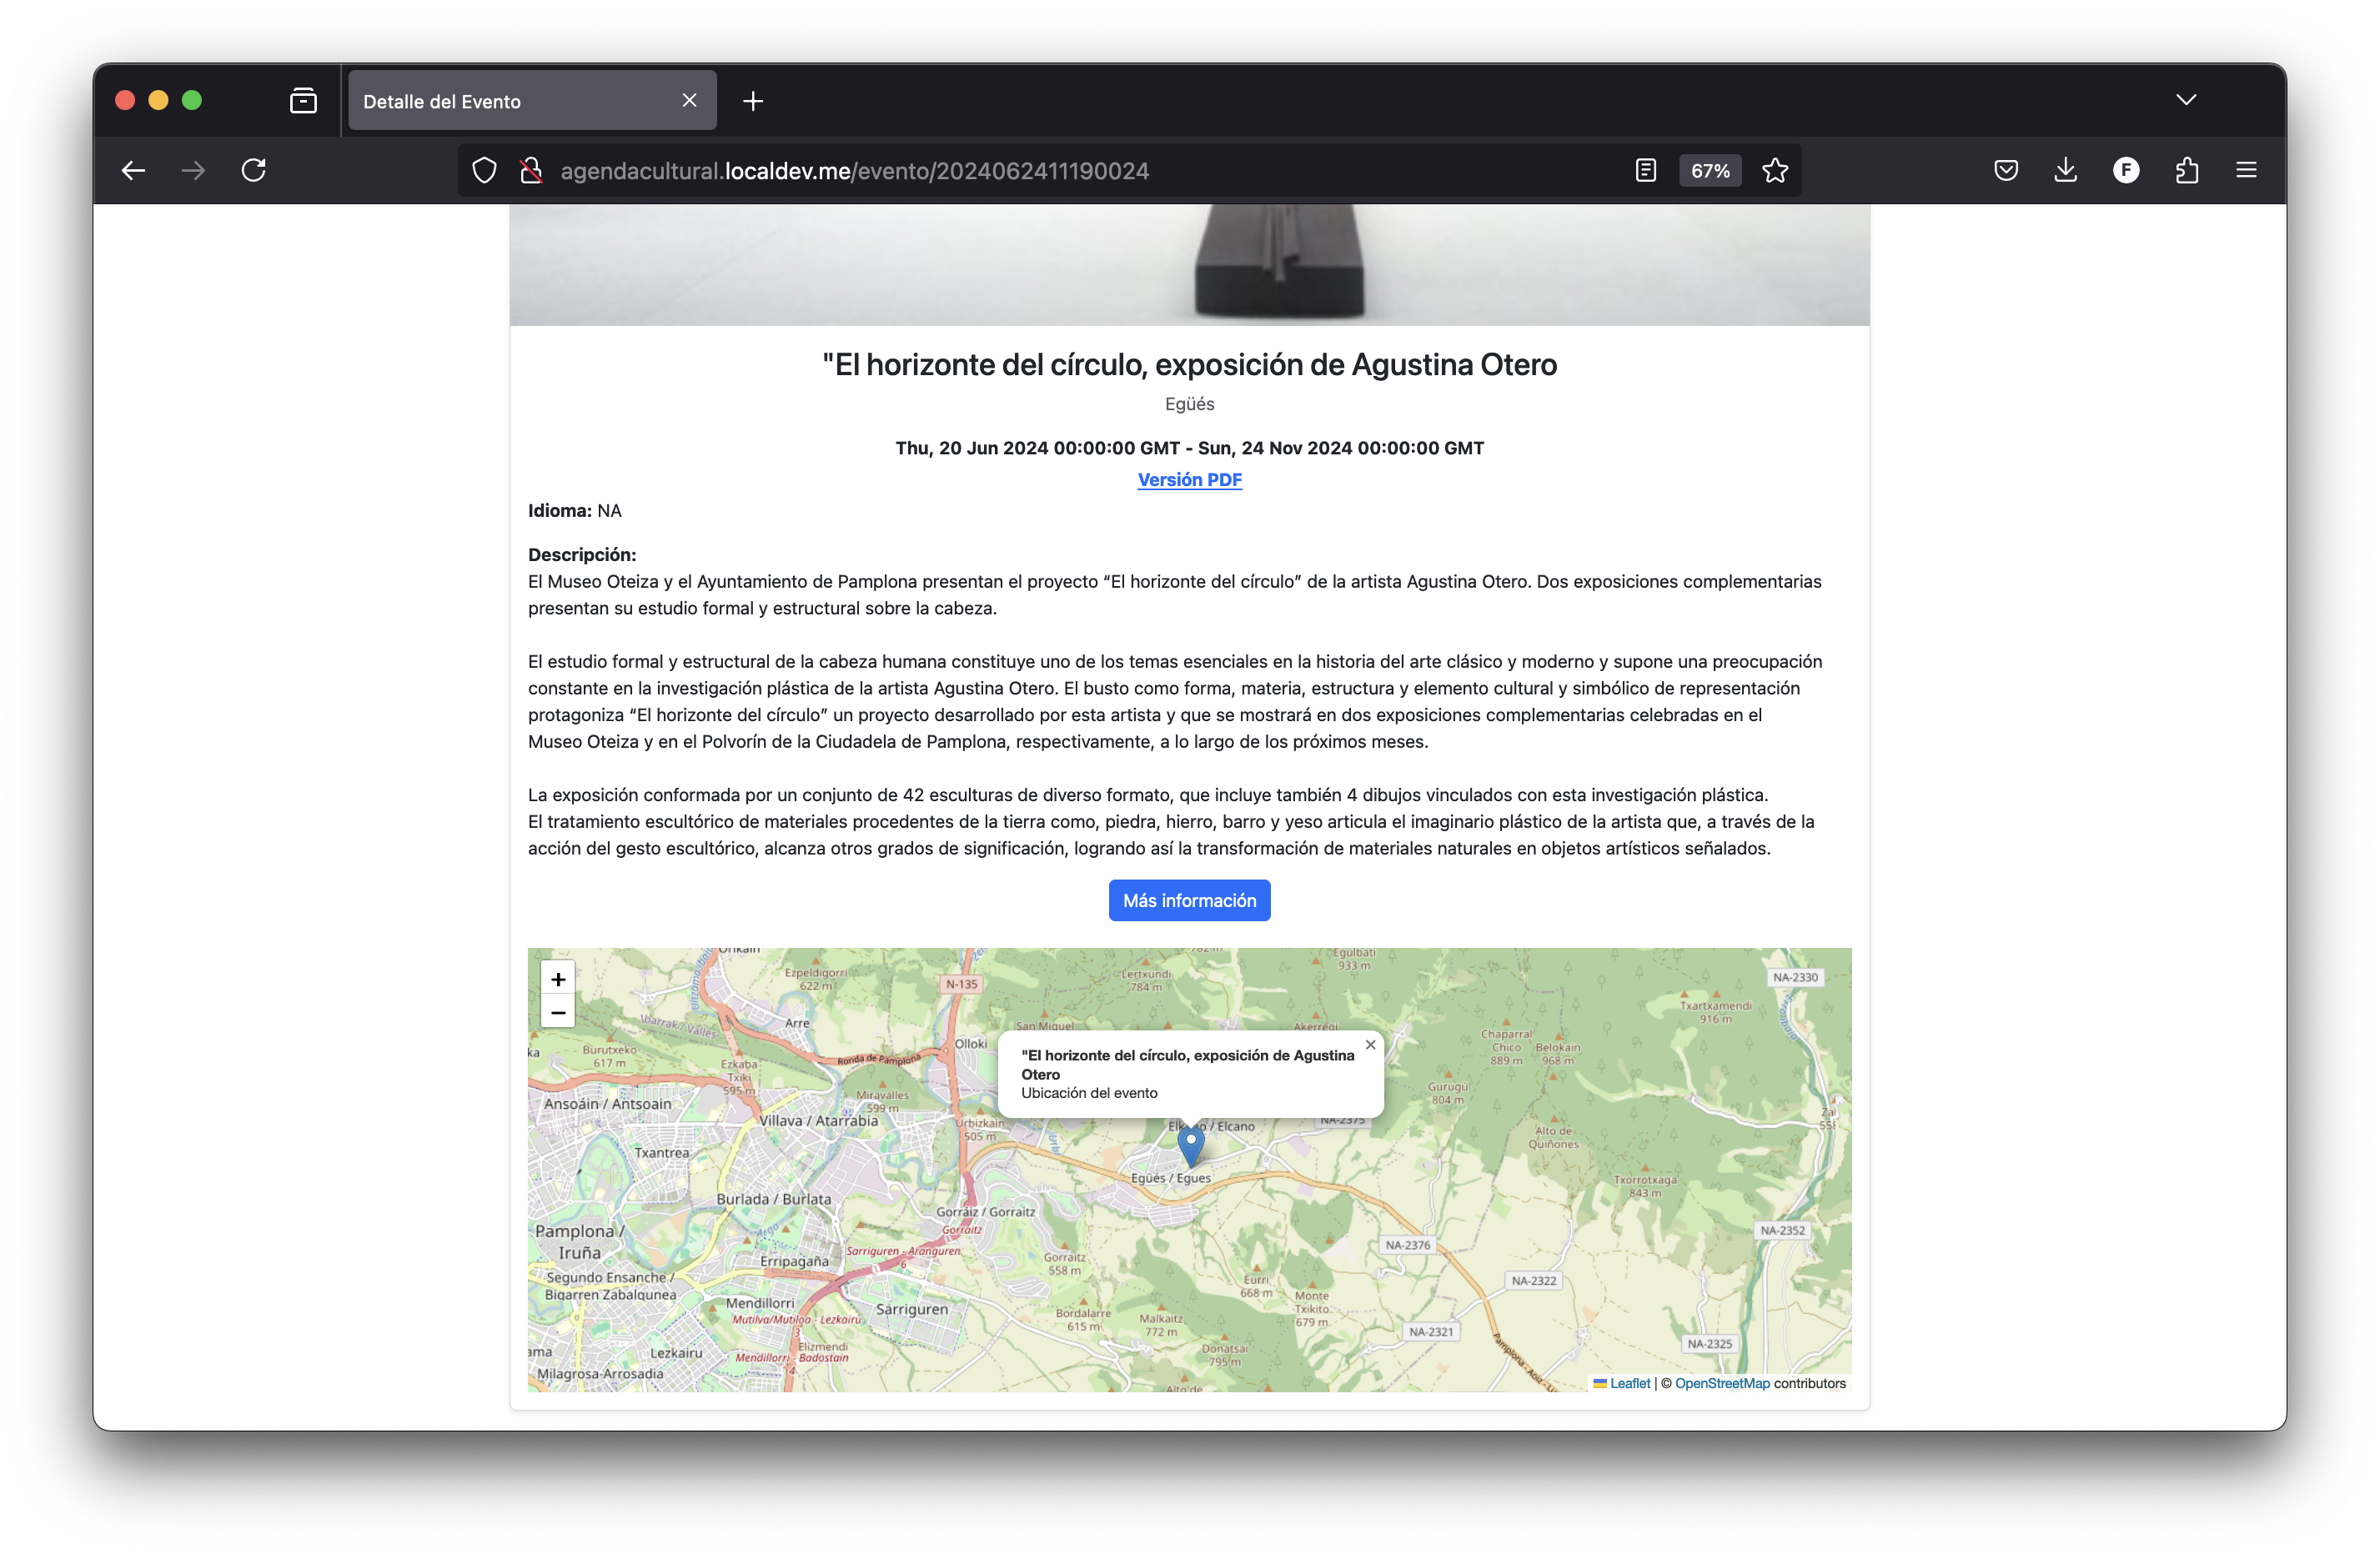
\includegraphics[width=0.9\linewidth]{img/manual-2.png}
            \caption{Ejemplo de detalle de un evento}
            \label{fig:manual-2}
        \end{figure}

        Por último, al presionar sobre el botón “PDF” de la página de inicio, o al presionar sobre el enlace “Versión PDF” dentro del detalle de un evento, se genera un documento PDF que, tal y como describe la \autoref{fig:manual-3}, muestra todos los detalles del evento, facilitando compartirlo o la impresión.

        \begin{figure}[H]
            \centering
            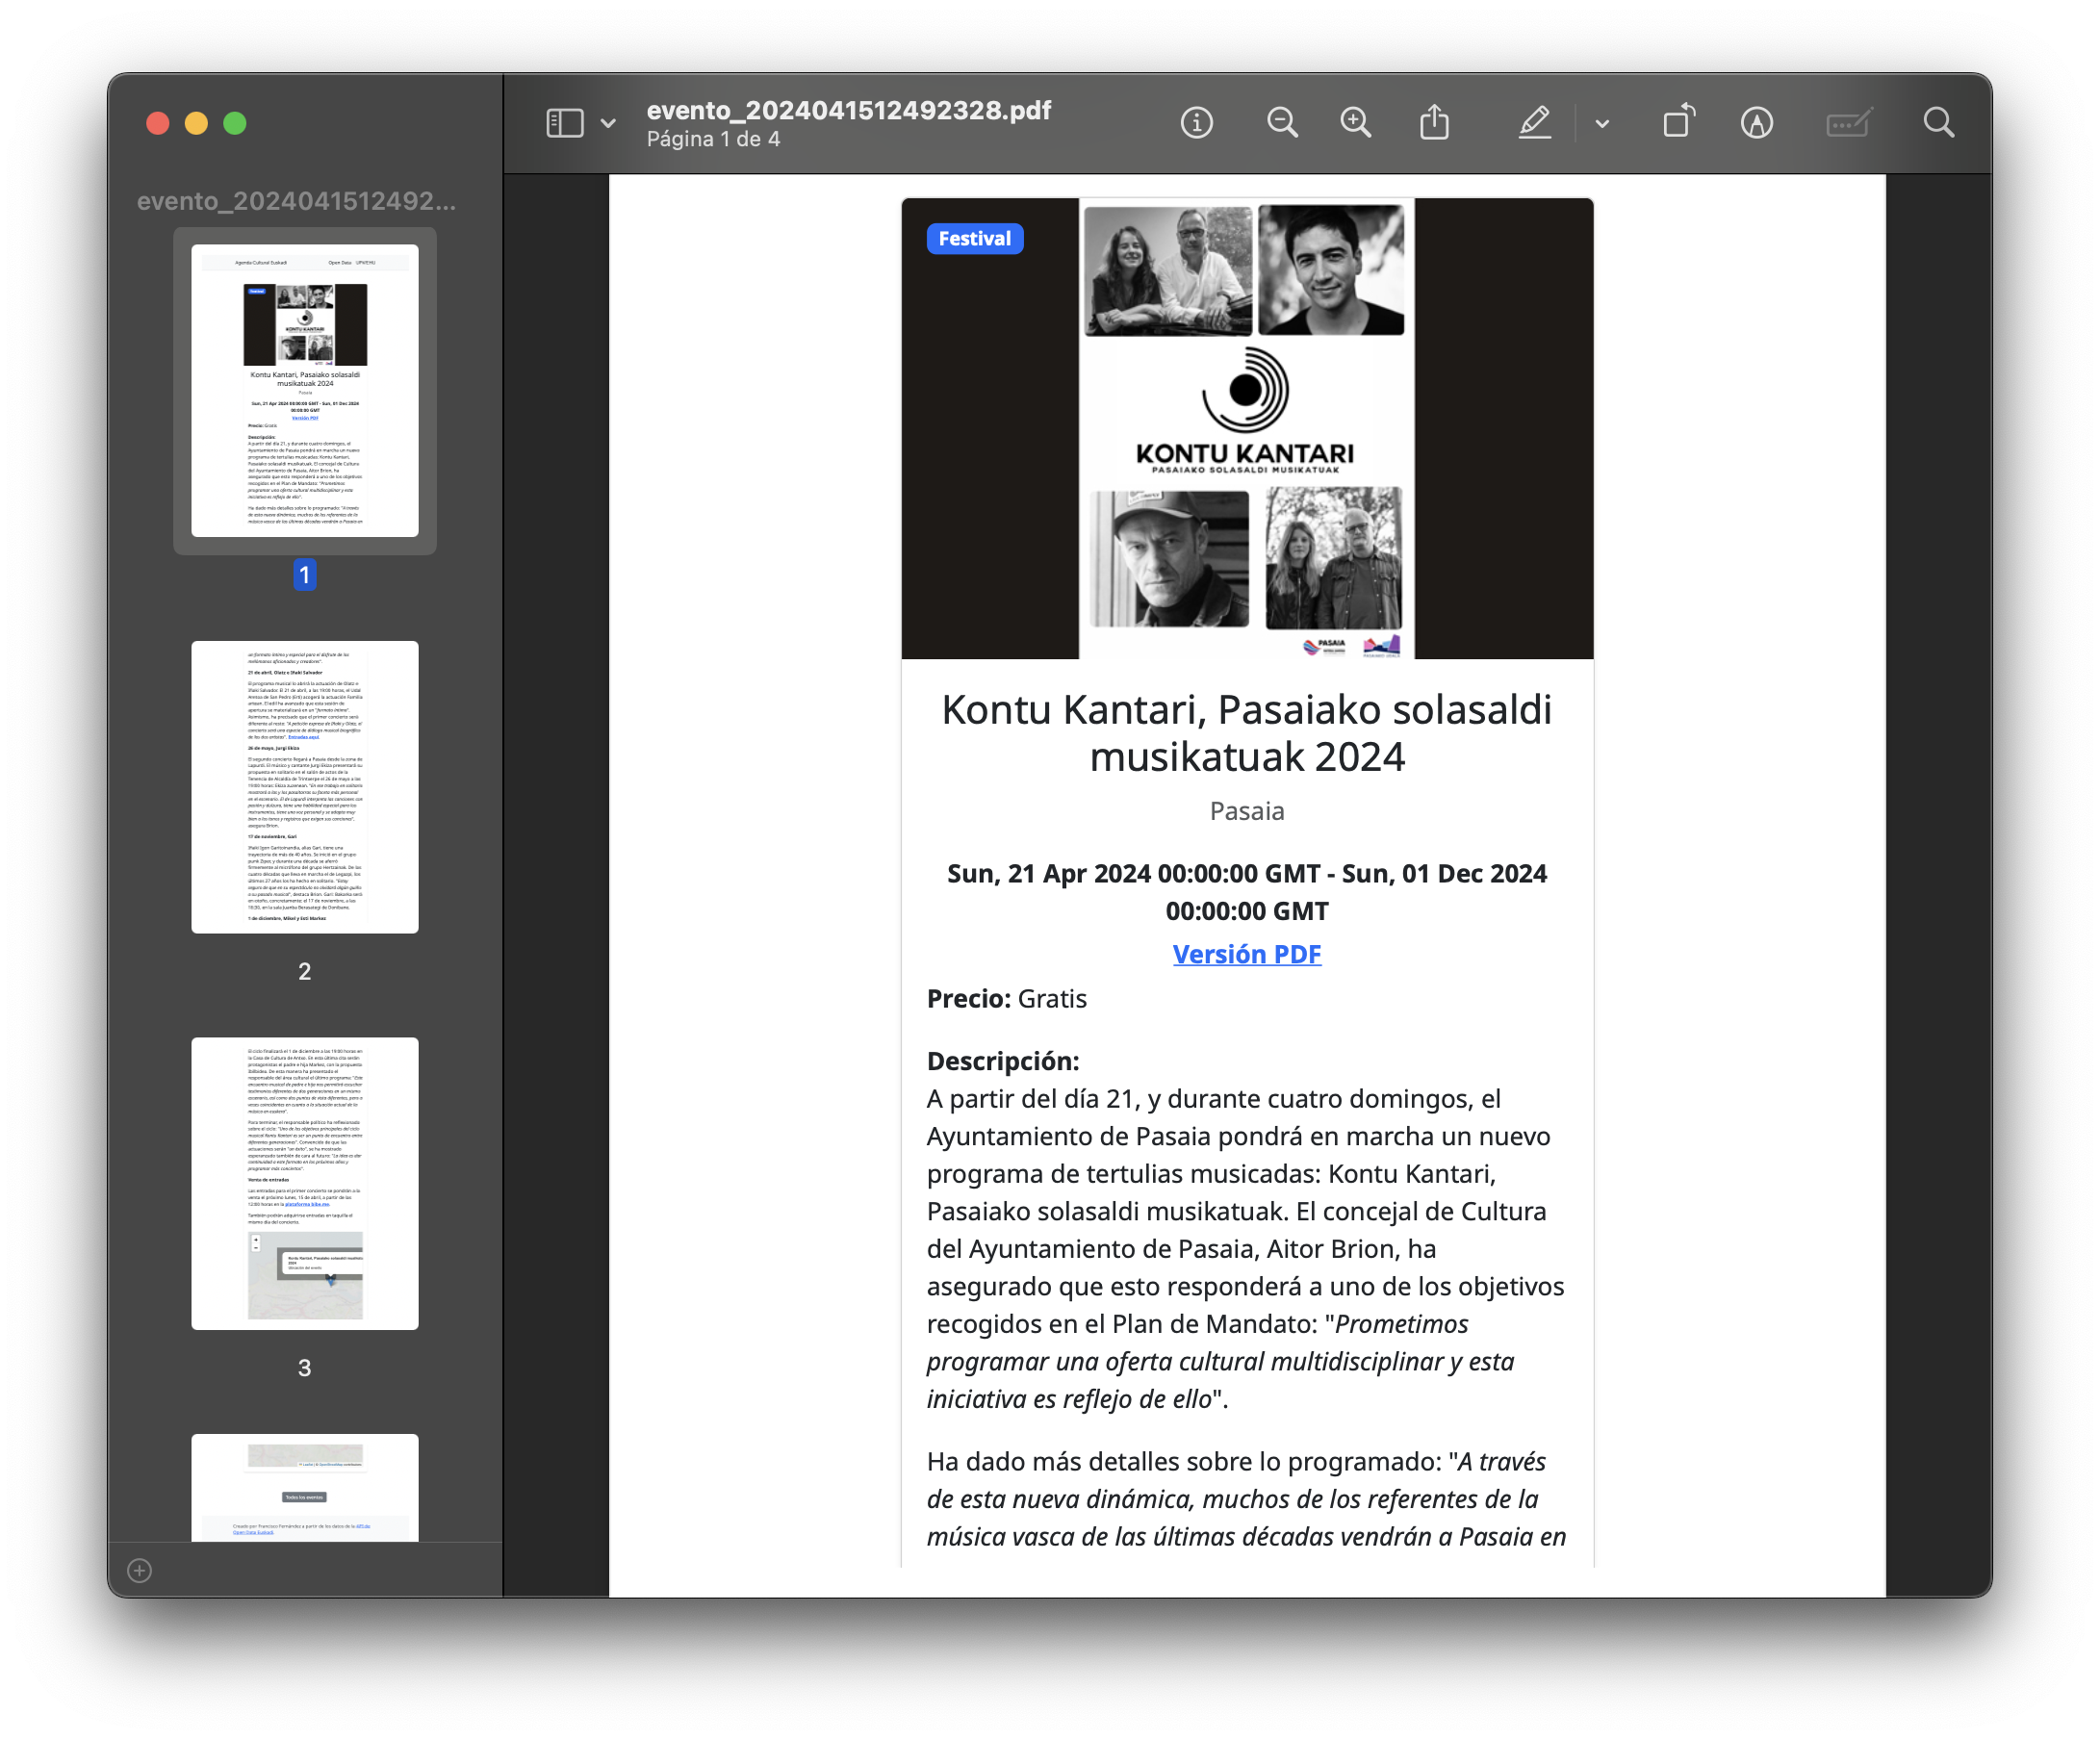
\includegraphics[width=0.65\linewidth]{img/manual-3.png}
            \caption{Ejemplo de documento PDF generado por la aplicación}
            \label{fig:manual-3}
        \end{figure}

    \chapter{Declaración sobre el uso de asistentes virtuales}

        Para la realización de este proyecto, se han utilizado en combinación los asistentes virtuales ChatGPT (OpenAI), Gemini (Google) y Copilot (Microsoft). No obstante, indicar en este caso que no han sido de ayuda en todo momento. Por ejemplo, la configuración de la tarea cron a partir de la imagen de Python de Docker ha tenido que crearse de forma manual a través de la información de múltiples repositorios de GitHub y preguntas de foros, pues ninguno de ellos sabía detallar cómo podían usarse librerías externas sobre el código. Tampoco gestionan bien el paso de Docker a Kubernetes, y proporcionan ficheros obsoletos, por ejemplo indicando la versión en Docker. No obstante, han sido de ayuda a la hora de optimizar tareas como el diseño, las consultas a la base de datos y, en general, para definir la estructura del proyecto.

    \clearpage
    \chapter{Bibliografía}
        \begin{itemize}
            \item \href{https://docs.docker.com}{\textit{Docker Docs}}.
            \item \href{https://github.com/adiii717/docker-python-cronjob/tree/master/cron-numpy}{\textit{adiii717/docker-python-cronjob/cron-numpy}}. GitHub.
            \item \href{https://es.stackoverflow.com/questions/564186/cron-en-un-dockerfile}{\textit{cron en un dockerfile}}. Stack Overflow en español.
            \item \href{https://www.adminer.org/}{\textit{Adminer.org}}.
            \item \href{https://medium.com/@habibullah.127.0.0.1/containerization-of-python-flask-nginx-in-docker-7c451b3328b7}{\textit{Containerization of Python Flask Nginx in docker}}. Medium (\textit{@habibullah.127.0.0.1}).
            \item \href{https://medium.com/@prashantsde/deploy-flask-app-inside-container-and-setup-nginx-reverse-proxy-ac4407fe07c}{\textit{Deploy flask app inside container and setup Nginx reverse proxy}}. Medium (\textit{@prashantsde}).
            \item \href{https://flask.palletsprojects.com/en/stable/tutorial/}{\textit{Flask Tutorial}}.
            \item \href{https://www.geeksforgeeks.org/python-build-a-rest-api-using-flask)/}{\textit{Python | Build a REST API using Flask}}. GeeksForGeeks.
            \item \href{https://gotenberg.dev/docs/getting-started/introduction}{\textit{Gotenberg Documentation}}.
            \item \href{https://kubernetes.io/docs/home/}{\textit{Kubernetes Documentation}}.
            \item \href{https://docs.docker.com/desktop/features/kubernetes/}{\textit{Deploy on Kubernetes with Docker Desktop}}. Docker Docs.
            \item \href{https://www.digitalocean.com/community/tutorials/how-to-deploy-postgres-to-kubernetes-cluster}{\textit{How to Deploy Postgres to Kubernetes Cluster}}. DigitalOcean Community.
            \item \href{https://www.cloudytuts.com/guides/kubernetes/how-to-deploy-postgress-kubernetes/}{\textit{How to Deploy Postgres on Kubernetes}}. CloudyTuts.
            \item \href{https://medium.com/@muppedaanvesh/a-hand-on-guide-to-kubernetes-cronjobs-%EF%B8%8F-47393a98716d}{\textit{A Hands-On Guide to Kubernetes CronJobs}}. Medium (\textit{@muppedaanvesh}).
            \item \href{https://www.geeksforgeeks.org/how-to-deploy-flask-app-on-kubernetes/}{\textit{How to Deploy Flask App on Kubernetes?}}. GeeksForGeeks.
        \end{itemize}

\end{document}
